\PassOptionsToPackage{unicode=true}{hyperref} % options for packages loaded elsewhere
\PassOptionsToPackage{hyphens}{url}
%
\documentclass[]{article}
\usepackage{lmodern}
\usepackage{amssymb,amsmath}
\usepackage{ifxetex,ifluatex}
\usepackage{fixltx2e} % provides \textsubscript
\ifnum 0\ifxetex 1\fi\ifluatex 1\fi=0 % if pdftex
  \usepackage[T1]{fontenc}
  \usepackage[utf8]{inputenc}
  \usepackage{textcomp} % provides euro and other symbols
\else % if luatex or xelatex
  \usepackage{unicode-math}
  \defaultfontfeatures{Ligatures=TeX,Scale=MatchLowercase}
\fi
% use upquote if available, for straight quotes in verbatim environments
\IfFileExists{upquote.sty}{\usepackage{upquote}}{}
% use microtype if available
\IfFileExists{microtype.sty}{%
\usepackage[]{microtype}
\UseMicrotypeSet[protrusion]{basicmath} % disable protrusion for tt fonts
}{}
\IfFileExists{parskip.sty}{%
\usepackage{parskip}
}{% else
\setlength{\parindent}{0pt}
\setlength{\parskip}{6pt plus 2pt minus 1pt}
}
\usepackage{hyperref}
\hypersetup{
            pdftitle={Multicollinearity: Question},
            pdfauthor={Thiyanga S. Talagala},
            pdfborder={0 0 0},
            breaklinks=true}
\urlstyle{same}  % don't use monospace font for urls
\usepackage[margin=1in]{geometry}
\usepackage{color}
\usepackage{fancyvrb}
\newcommand{\VerbBar}{|}
\newcommand{\VERB}{\Verb[commandchars=\\\{\}]}
\DefineVerbatimEnvironment{Highlighting}{Verbatim}{commandchars=\\\{\}}
% Add ',fontsize=\small' for more characters per line
\usepackage{framed}
\definecolor{shadecolor}{RGB}{248,248,248}
\newenvironment{Shaded}{\begin{snugshade}}{\end{snugshade}}
\newcommand{\AlertTok}[1]{\textcolor[rgb]{0.94,0.16,0.16}{#1}}
\newcommand{\AnnotationTok}[1]{\textcolor[rgb]{0.56,0.35,0.01}{\textbf{\textit{#1}}}}
\newcommand{\AttributeTok}[1]{\textcolor[rgb]{0.77,0.63,0.00}{#1}}
\newcommand{\BaseNTok}[1]{\textcolor[rgb]{0.00,0.00,0.81}{#1}}
\newcommand{\BuiltInTok}[1]{#1}
\newcommand{\CharTok}[1]{\textcolor[rgb]{0.31,0.60,0.02}{#1}}
\newcommand{\CommentTok}[1]{\textcolor[rgb]{0.56,0.35,0.01}{\textit{#1}}}
\newcommand{\CommentVarTok}[1]{\textcolor[rgb]{0.56,0.35,0.01}{\textbf{\textit{#1}}}}
\newcommand{\ConstantTok}[1]{\textcolor[rgb]{0.00,0.00,0.00}{#1}}
\newcommand{\ControlFlowTok}[1]{\textcolor[rgb]{0.13,0.29,0.53}{\textbf{#1}}}
\newcommand{\DataTypeTok}[1]{\textcolor[rgb]{0.13,0.29,0.53}{#1}}
\newcommand{\DecValTok}[1]{\textcolor[rgb]{0.00,0.00,0.81}{#1}}
\newcommand{\DocumentationTok}[1]{\textcolor[rgb]{0.56,0.35,0.01}{\textbf{\textit{#1}}}}
\newcommand{\ErrorTok}[1]{\textcolor[rgb]{0.64,0.00,0.00}{\textbf{#1}}}
\newcommand{\ExtensionTok}[1]{#1}
\newcommand{\FloatTok}[1]{\textcolor[rgb]{0.00,0.00,0.81}{#1}}
\newcommand{\FunctionTok}[1]{\textcolor[rgb]{0.00,0.00,0.00}{#1}}
\newcommand{\ImportTok}[1]{#1}
\newcommand{\InformationTok}[1]{\textcolor[rgb]{0.56,0.35,0.01}{\textbf{\textit{#1}}}}
\newcommand{\KeywordTok}[1]{\textcolor[rgb]{0.13,0.29,0.53}{\textbf{#1}}}
\newcommand{\NormalTok}[1]{#1}
\newcommand{\OperatorTok}[1]{\textcolor[rgb]{0.81,0.36,0.00}{\textbf{#1}}}
\newcommand{\OtherTok}[1]{\textcolor[rgb]{0.56,0.35,0.01}{#1}}
\newcommand{\PreprocessorTok}[1]{\textcolor[rgb]{0.56,0.35,0.01}{\textit{#1}}}
\newcommand{\RegionMarkerTok}[1]{#1}
\newcommand{\SpecialCharTok}[1]{\textcolor[rgb]{0.00,0.00,0.00}{#1}}
\newcommand{\SpecialStringTok}[1]{\textcolor[rgb]{0.31,0.60,0.02}{#1}}
\newcommand{\StringTok}[1]{\textcolor[rgb]{0.31,0.60,0.02}{#1}}
\newcommand{\VariableTok}[1]{\textcolor[rgb]{0.00,0.00,0.00}{#1}}
\newcommand{\VerbatimStringTok}[1]{\textcolor[rgb]{0.31,0.60,0.02}{#1}}
\newcommand{\WarningTok}[1]{\textcolor[rgb]{0.56,0.35,0.01}{\textbf{\textit{#1}}}}
\usepackage{graphicx,grffile}
\makeatletter
\def\maxwidth{\ifdim\Gin@nat@width>\linewidth\linewidth\else\Gin@nat@width\fi}
\def\maxheight{\ifdim\Gin@nat@height>\textheight\textheight\else\Gin@nat@height\fi}
\makeatother
% Scale images if necessary, so that they will not overflow the page
% margins by default, and it is still possible to overwrite the defaults
% using explicit options in \includegraphics[width, height, ...]{}
\setkeys{Gin}{width=\maxwidth,height=\maxheight,keepaspectratio}
\setlength{\emergencystretch}{3em}  % prevent overfull lines
\providecommand{\tightlist}{%
  \setlength{\itemsep}{0pt}\setlength{\parskip}{0pt}}
\setcounter{secnumdepth}{0}
% Redefines (sub)paragraphs to behave more like sections
\ifx\paragraph\undefined\else
\let\oldparagraph\paragraph
\renewcommand{\paragraph}[1]{\oldparagraph{#1}\mbox{}}
\fi
\ifx\subparagraph\undefined\else
\let\oldsubparagraph\subparagraph
\renewcommand{\subparagraph}[1]{\oldsubparagraph{#1}\mbox{}}
\fi

% set default figure placement to htbp
\makeatletter
\def\fps@figure{htbp}
\makeatother

\usepackage{etoolbox}
\makeatletter
\providecommand{\subtitle}[1]{% add subtitle to \maketitle
  \apptocmd{\@title}{\par {\large #1 \par}}{}{}
}
\makeatother

\title{Multicollinearity: Question}
\providecommand{\subtitle}[1]{}
\subtitle{STA 506 2.0 Linear Regression Analysis}
\author{Thiyanga S. Talagala}
\date{}

\begin{document}
\maketitle

\hypertarget{data}{%
\subsection{Data}\label{data}}

\begin{Shaded}
\begin{Highlighting}[]
\KeywordTok{library}\NormalTok{(tidyverse)}
\NormalTok{realestate <-}\StringTok{ }\KeywordTok{read.csv}\NormalTok{(}\StringTok{"real-estate.csv"}\NormalTok{)}
\KeywordTok{head}\NormalTok{(realestate)}
\end{Highlighting}
\end{Shaded}

\begin{verbatim}
  ID  Price Sqft Bedroom Bathroom Airconditioning Garage Pool YearBuild Quality
1  1 360000 3032       4        4               1      2    0      1972       2
2  2 340000 2058       4        2               1      2    0      1976       2
3  3 250000 1780       4        3               1      2    0      1980       2
4  4 205500 1638       4        2               1      2    0      1963       2
5  5 275500 2196       4        3               1      2    0      1968       2
6  6 248000 1966       4        3               1      5    1      1972       2
    Lot AdjHighway
1 22221          0
2 22912          0
3 21345          0
4 17342          0
5 21786          0
6 18902          0
\end{verbatim}

\begin{Shaded}
\begin{Highlighting}[]
\KeywordTok{glimpse}\NormalTok{(realestate)}
\end{Highlighting}
\end{Shaded}

\begin{verbatim}
Rows: 522
Columns: 12
$ ID              <int> 1, 2, 3, 4, 5, 6, 7, 8, 9, 10, 11, 12, 13, 14, 15, ...
$ Price           <int> 360000, 340000, 250000, 205500, 275500, 248000, 229...
$ Sqft            <int> 3032, 2058, 1780, 1638, 2196, 1966, 2216, 1597, 162...
$ Bedroom         <int> 4, 4, 4, 4, 4, 4, 3, 2, 3, 3, 7, 3, 5, 5, 3, 5, 2, ...
$ Bathroom        <int> 4, 2, 3, 2, 3, 3, 2, 1, 2, 3, 5, 4, 4, 4, 3, 5, 2, ...
$ Airconditioning <int> 1, 1, 1, 1, 1, 1, 1, 1, 1, 0, 0, 1, 1, 1, 1, 1, 1, ...
$ Garage          <int> 2, 2, 2, 2, 2, 5, 2, 1, 2, 1, 2, 3, 3, 2, 2, 2, 2, ...
$ Pool            <int> 0, 0, 0, 0, 0, 1, 0, 0, 0, 0, 1, 0, 0, 0, 0, 0, 0, ...
$ YearBuild       <int> 1972, 1976, 1980, 1963, 1968, 1972, 1972, 1955, 197...
$ Quality         <int> 2, 2, 2, 2, 2, 2, 2, 2, 3, 3, 3, 1, 1, 1, 2, 2, 2, ...
$ Lot             <int> 22221, 22912, 21345, 17342, 21786, 18902, 18639, 22...
$ AdjHighway      <int> 0, 0, 0, 0, 0, 0, 0, 0, 0, 0, 0, 0, 0, 0, 0, 0, 0, ...
\end{verbatim}

\newpage

\hypertarget{q1-identify-qualitative-and-quantitative-variables.}{%
\subsection{Q1: Identify qualitative and quantitative
variables.}\label{q1-identify-qualitative-and-quantitative-variables.}}

\begin{verbatim}
       ID            Price             Sqft         Bedroom     
 Min.   :  1.0   Min.   : 84000   Min.   : 980   Min.   :0.000  
 1st Qu.:131.2   1st Qu.:180000   1st Qu.:1701   1st Qu.:3.000  
 Median :261.5   Median :229900   Median :2061   Median :3.000  
 Mean   :261.5   Mean   :277894   Mean   :2261   Mean   :3.471  
 3rd Qu.:391.8   3rd Qu.:335000   3rd Qu.:2636   3rd Qu.:4.000  
 Max.   :522.0   Max.   :920000   Max.   :5032   Max.   :7.000  
    Bathroom     Airconditioning     Garage    Pool      YearBuild    Quality
 Min.   :0.000   0: 88           Min.   :0.0   0:486   Min.   :1885   1: 68  
 1st Qu.:2.000   1:434           1st Qu.:2.0   1: 36   1st Qu.:1956   2:290  
 Median :3.000                   Median :2.0           Median :1966   3:164  
 Mean   :2.642                   Mean   :2.1           Mean   :1967          
 3rd Qu.:3.000                   3rd Qu.:2.0           3rd Qu.:1981          
 Max.   :7.000                   Max.   :7.0           Max.   :1998          
      Lot        AdjHighway
 Min.   : 4560   0:511     
 1st Qu.:17205   1: 11     
 Median :22200             
 Mean   :24370             
 3rd Qu.:26787             
 Max.   :86830             
\end{verbatim}

\newpage

\hypertarget{q2-what-is-wrong-with-the-following-graph}{%
\subsection{Q2: What is wrong with the following
graph?}\label{q2-what-is-wrong-with-the-following-graph}}

\begin{figure}
\centering
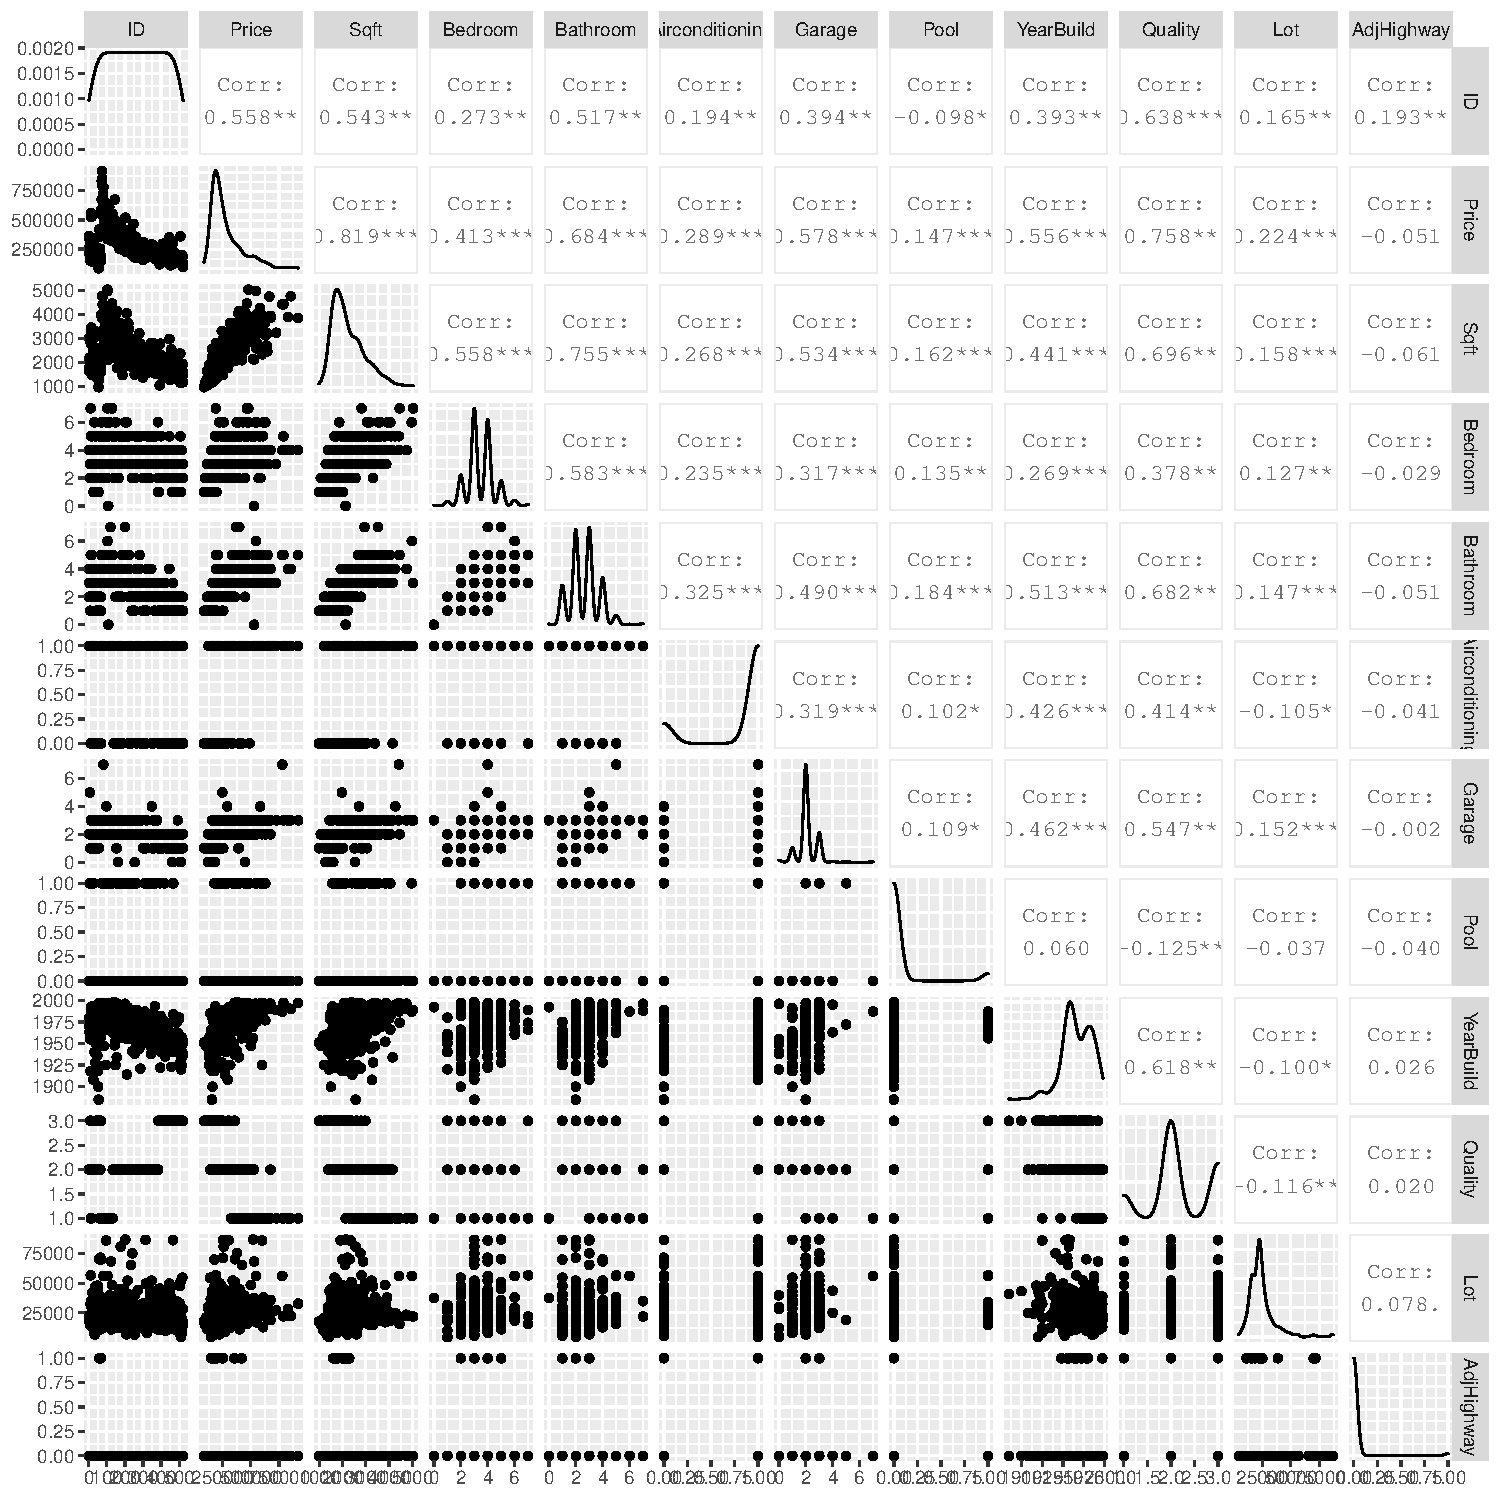
\includegraphics{multicollinearity_questions_files/figure-latex/unnamed-chunk-4-1.pdf}
\caption{Pairwise correlation plot}
\end{figure}

\newpage

\hypertarget{q3-figure-1-is-modified-as-follows.-now-what-can-you-say-about-the-graph}{%
\subsection{Q3: Figure 1 is modified as follows. Now what can you say
about the
graph?}\label{q3-figure-1-is-modified-as-follows.-now-what-can-you-say-about-the-graph}}

\begin{figure}
\centering
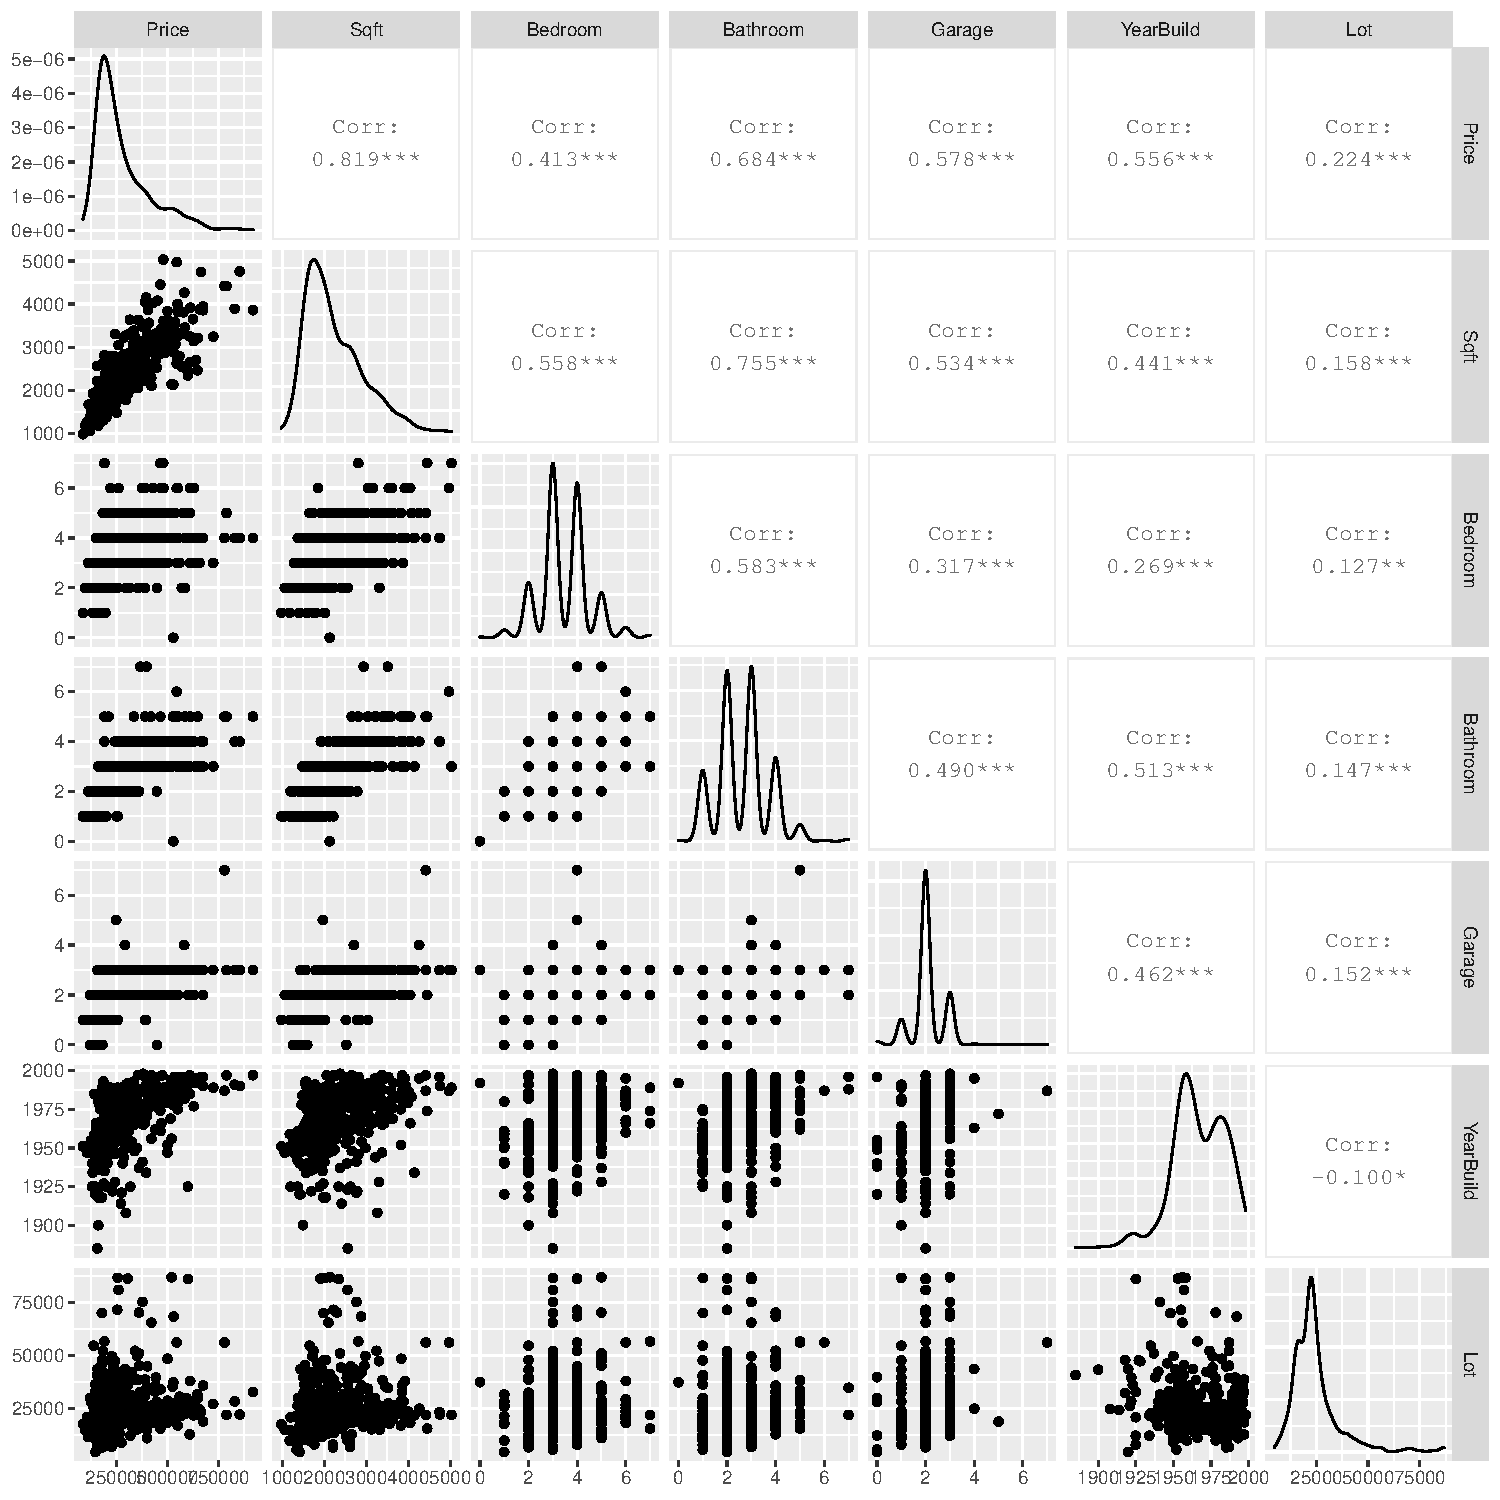
\includegraphics{multicollinearity_questions_files/figure-latex/unnamed-chunk-5-1.pdf}
\caption{Pairwise correlation plot}
\end{figure}

\newpage

\hypertarget{q4-what-can-you-say-about-the-source-of-multicollinearity-in-these-data}{%
\subsection{Q4: What can you say about the source of multicollinearity
in these
data?}\label{q4-what-can-you-say-about-the-source-of-multicollinearity-in-these-data}}

\begin{Shaded}
\begin{Highlighting}[]
\NormalTok{realestate}\OperatorTok{$}\NormalTok{Airconditioning <-}\StringTok{ }\KeywordTok{factor}\NormalTok{(realestate}\OperatorTok{$}\NormalTok{Airconditioning)}
\NormalTok{realestate}\OperatorTok{$}\NormalTok{Pool <-}\StringTok{ }\KeywordTok{factor}\NormalTok{(realestate}\OperatorTok{$}\NormalTok{Pool)}
\NormalTok{realestate}\OperatorTok{$}\NormalTok{AdjHighway <-}\StringTok{ }\KeywordTok{factor}\NormalTok{(realestate}\OperatorTok{$}\NormalTok{AdjHighway)}
\NormalTok{realestate}\OperatorTok{$}\NormalTok{Quality <-}\StringTok{ }\KeywordTok{factor}\NormalTok{(realestate}\OperatorTok{$}\NormalTok{Quality)}
\NormalTok{realestate <-}\StringTok{ }\NormalTok{realestate[, }\DecValTok{-1}\NormalTok{]}
\KeywordTok{summary}\NormalTok{(realestate)}
\end{Highlighting}
\end{Shaded}

\begin{verbatim}
     Price             Sqft         Bedroom         Bathroom    
 Min.   : 84000   Min.   : 980   Min.   :0.000   Min.   :0.000  
 1st Qu.:180000   1st Qu.:1701   1st Qu.:3.000   1st Qu.:2.000  
 Median :229900   Median :2061   Median :3.000   Median :3.000  
 Mean   :277894   Mean   :2261   Mean   :3.471   Mean   :2.642  
 3rd Qu.:335000   3rd Qu.:2636   3rd Qu.:4.000   3rd Qu.:3.000  
 Max.   :920000   Max.   :5032   Max.   :7.000   Max.   :7.000  
 Airconditioning     Garage    Pool      YearBuild    Quality      Lot       
 0: 88           Min.   :0.0   0:486   Min.   :1885   1: 68   Min.   : 4560  
 1:434           1st Qu.:2.0   1: 36   1st Qu.:1956   2:290   1st Qu.:17205  
                 Median :2.0           Median :1966   3:164   Median :22200  
                 Mean   :2.1           Mean   :1967           Mean   :24370  
                 3rd Qu.:2.0           3rd Qu.:1981           3rd Qu.:26787  
                 Max.   :7.0           Max.   :1998           Max.   :86830  
 AdjHighway
 0:511     
 1: 11     
           
           
           
           
\end{verbatim}

\begin{Shaded}
\begin{Highlighting}[]
\NormalTok{model <-}\StringTok{ }\KeywordTok{lm}\NormalTok{(Price }\OperatorTok{~}\StringTok{ }\NormalTok{. , }\DataTypeTok{data=}\NormalTok{realestate)}
\KeywordTok{summary}\NormalTok{(model)}
\end{Highlighting}
\end{Shaded}

\begin{verbatim}

Call:
lm(formula = Price ~ ., data = realestate)

Residuals:
    Min      1Q  Median      3Q     Max 
-204865  -28010   -4973   21315  298892 

Coefficients:
                   Estimate Std. Error t value Pr(>|t|)    
(Intercept)      -2.358e+06  3.991e+05  -5.909 6.29e-09 ***
Sqft              8.700e+01  6.570e+00  13.242  < 2e-16 ***
Bedroom          -5.125e+03  3.275e+03  -1.565   0.1182    
Bathroom          8.127e+03  4.288e+03   1.895   0.0586 .  
Airconditioning1  4.851e+03  8.086e+03   0.600   0.5488    
Garage            1.089e+04  5.060e+03   2.152   0.0319 *  
Pool1             1.014e+04  1.040e+04   0.975   0.3303    
YearBuild         1.269e+03  2.024e+02   6.272 7.60e-10 ***
Quality2         -1.430e+05  1.021e+04 -14.007  < 2e-16 ***
Quality3         -1.484e+05  1.404e+04 -10.564  < 2e-16 ***
Lot               1.556e+00  2.363e-01   6.587 1.12e-10 ***
AdjHighway1      -2.737e+04  1.810e+04  -1.512   0.1311    
---
Signif. codes:  0 '***' 0.001 '**' 0.01 '*' 0.05 '.' 0.1 ' ' 1

Residual standard error: 58770 on 510 degrees of freedom
Multiple R-squared:  0.8223,    Adjusted R-squared:  0.8184 
F-statistic: 214.5 on 11 and 510 DF,  p-value: < 2.2e-16
\end{verbatim}

\begin{Shaded}
\begin{Highlighting}[]
\KeywordTok{library}\NormalTok{(car)}
\NormalTok{car}\OperatorTok{::}\KeywordTok{vif}\NormalTok{(model)}
\end{Highlighting}
\end{Shaded}

\begin{verbatim}
                    GVIF Df GVIF^(1/(2*Df))
Sqft            3.292569  1        1.814544
Bedroom         1.664845  1        1.290289
Bathroom        3.141563  1        1.772445
Airconditioning 1.385038  1        1.176876
Garage          1.651938  1        1.285277
Pool            1.050442  1        1.024911
YearBuild       1.922344  1        1.386486
Quality         3.322305  2        1.350081
Lot             1.150133  1        1.072443
AdjHighway      1.021444  1        1.010665
\end{verbatim}

\newpage

\hypertarget{note}{%
\section{Note:}\label{note}}

\hypertarget{note-1}{%
\subsection{1.1: note}\label{note-1}}

Multicollinearity occurs if we do not treat this appropriately.

\hypertarget{model-with-only-quantitative-variables-vif}{%
\subsubsection{1.2 Model with only quantitative variables:
VIF}\label{model-with-only-quantitative-variables-vif}}

\begin{Shaded}
\begin{Highlighting}[]
\KeywordTok{summary}\NormalTok{(Duncan)}
\end{Highlighting}
\end{Shaded}

\begin{verbatim}
   type        income        education         prestige    
 bc  :21   Min.   : 7.00   Min.   :  7.00   Min.   : 3.00  
 prof:18   1st Qu.:21.00   1st Qu.: 26.00   1st Qu.:16.00  
 wc  : 6   Median :42.00   Median : 45.00   Median :41.00  
           Mean   :41.87   Mean   : 52.56   Mean   :47.69  
           3rd Qu.:64.00   3rd Qu.: 84.00   3rd Qu.:81.00  
           Max.   :81.00   Max.   :100.00   Max.   :97.00  
\end{verbatim}

\begin{Shaded}
\begin{Highlighting}[]
\NormalTok{m1 <-}\StringTok{ }\KeywordTok{lm}\NormalTok{(prestige }\OperatorTok{~}\StringTok{ }\NormalTok{income }\OperatorTok{+}\StringTok{ }\NormalTok{education, }\DataTypeTok{data=}\NormalTok{Duncan)}
\KeywordTok{vif}\NormalTok{(m1)}
\end{Highlighting}
\end{Shaded}

\begin{verbatim}
   income education 
   2.1049    2.1049 
\end{verbatim}

\hypertarget{model-with-only-quantitative-variables-and-qualitative-variables-generalized-variance-inflation-factors}{%
\subsubsection{1.3 Model with only quantitative variables and
qualitative variables: Generalized variance-inflation
factors}\label{model-with-only-quantitative-variables-and-qualitative-variables-generalized-variance-inflation-factors}}

\begin{Shaded}
\begin{Highlighting}[]
\NormalTok{m2 <-}\StringTok{ }\KeywordTok{lm}\NormalTok{(prestige }\OperatorTok{~}\StringTok{ }\NormalTok{income }\OperatorTok{+}\StringTok{ }\NormalTok{education }\OperatorTok{+}\StringTok{ }\NormalTok{type, }\DataTypeTok{data=}\NormalTok{Duncan)}
\KeywordTok{vif}\NormalTok{(m2)}
\end{Highlighting}
\end{Shaded}

\begin{verbatim}
              GVIF Df GVIF^(1/(2*Df))
income    2.209178  1        1.486330
education 5.297584  1        2.301648
type      5.098592  2        1.502666
\end{verbatim}

\newpage

\newpage

\hypertarget{q5-write-down-the-estimated-model.}{%
\subsection{Q5: Write down the estimated
model.}\label{q5-write-down-the-estimated-model.}}

\begin{Shaded}
\begin{Highlighting}[]
\KeywordTok{summary}\NormalTok{(model)}
\end{Highlighting}
\end{Shaded}

\begin{verbatim}

Call:
lm(formula = Price ~ ., data = realestate)

Residuals:
    Min      1Q  Median      3Q     Max 
-204865  -28010   -4973   21315  298892 

Coefficients:
                   Estimate Std. Error t value Pr(>|t|)    
(Intercept)      -2.358e+06  3.991e+05  -5.909 6.29e-09 ***
Sqft              8.700e+01  6.570e+00  13.242  < 2e-16 ***
Bedroom          -5.125e+03  3.275e+03  -1.565   0.1182    
Bathroom          8.127e+03  4.288e+03   1.895   0.0586 .  
Airconditioning1  4.851e+03  8.086e+03   0.600   0.5488    
Garage            1.089e+04  5.060e+03   2.152   0.0319 *  
Pool1             1.014e+04  1.040e+04   0.975   0.3303    
YearBuild         1.269e+03  2.024e+02   6.272 7.60e-10 ***
Quality2         -1.430e+05  1.021e+04 -14.007  < 2e-16 ***
Quality3         -1.484e+05  1.404e+04 -10.564  < 2e-16 ***
Lot               1.556e+00  2.363e-01   6.587 1.12e-10 ***
AdjHighway1      -2.737e+04  1.810e+04  -1.512   0.1311    
---
Signif. codes:  0 '***' 0.001 '**' 0.01 '*' 0.05 '.' 0.1 ' ' 1

Residual standard error: 58770 on 510 degrees of freedom
Multiple R-squared:  0.8223,    Adjusted R-squared:  0.8184 
F-statistic: 214.5 on 11 and 510 DF,  p-value: < 2.2e-16
\end{verbatim}

\newpage

\end{document}
